\documentclass[10pt,letterpaper]{article}
\usepackage[T1]{fontenc}
\usepackage{lmodern}
\usepackage[letterpaper,margin=1in]{geometry}
\usepackage{amsmath,amssymb,booktabs,graphicx,url}
\usepackage[hidelinks]{hyperref}
\usepackage[labelfont=normalfont,font=small,skip=5pt]{caption}
\setlength{\textfloatsep}{11pt plus 2pt minus 2pt}
\setlength{\floatsep}{9pt plus 2pt minus 2pt}
\setlength{\intextsep}{9pt plus 2pt minus 2pt}

\renewcommand{\thesection}{S\arabic{section}}
\renewcommand{\thesubsection}{S\arabic{section}.\arabic{subsection}}
\renewcommand{\theequation}{S\arabic{equation}}
\renewcommand{\thetable}{S\arabic{table}}
\renewcommand{\thefigure}{S\arabic{figure}}

\newcommand{\ci}[2]{\shortstack{#1\\{}[#2]}}

\hypersetup{
  pdftitle={Supplementary Material - NeST-Com: Fixed-Budget Next-Scale Token Communication},
  pdfauthor={Lu Liu, Lifang Feng, Jianping Wang, Hongyao Chen, Huimin Lu}
}

\begin{document}

\begin{center}
{\Large Supplementary Material}\\[4pt]
{\large NeST-Com: Fixed-Budget Next-Scale Token Communication}\\[6pt]
{\normalsize Lu Liu, Lifang Feng\textsuperscript{*}, Jianping Wang, Hongyao Chen, and Huimin Lu}\\[2pt]
{\small University of Science and Technology Beijing, Beijing, China}\\
{\small \textsuperscript{*}Corresponding author: Lifang Feng (\href{mailto:lffeng@ustb.edu.cn}{\nolinkurl{lffeng@ustb.edu.cn}})}
\end{center}

\vspace{4pt}
\noindent This document provides the complete coding algorithm and its nondecreasing-length proof (Section~S1), controlled ablations on receiver reconstruction and endpoint granularity (Section~S2), extended fixed-budget, equal-information, and cross-dataset reconstruction tables (Section~S3), and channel-threshold, latency, and qualitative analyses (Section~S4). Notation follows the main manuscript, and all paired differences and relative gains are computed from unrounded source-level values prior to rounding.

\section{Algorithm and Experimental Protocol}

\subsection{Independent prefix decoding and frame fitting}
The shared frozen VAR tokenizer decomposes a $256\times 256$ image into ten residual token maps with spatial side lengths $(1,2,3,4,5,6,8,10,13,16)$ over a $4096$-entry codebook. An endpoint $(m,K)$ retains the first $m$ complete maps together with the first $K$ raster-ordered positions of map $m+1$. Whereas WHOLE restricts truncation to complete-map boundaries, NeST admits all $651$ within-scale endpoints spanning $30$--$680$ tokens; the coarser Quarter and Eighth grids restrict partial-map endpoints to $\lfloor jL/d\rfloor$ ($j=1,\ldots,d-1$, with $d=4$ and $8$, respectively) alongside complete-map boundaries.

Because token probabilities at any scale depend exclusively on complete coarser maps, both transmitter and receiver construct identical entropy-coding contexts from the recovered prefix without transmitting side probabilities or unreceived tokens. Let $\ell_j$ denote the FP32 log-softmax output, with codebook size $V=4096$ and total frequency $M=2^{24}$. Positive integer symbol frequencies are formed as
\begin{align}
p_j &= \frac{\exp(\ell_j - \max_k \ell_k)}{\sum_k \exp(\ell_k - \max_k \ell_k)}, &
f_j &= \lfloor p_j(M - V)\rfloor + 1, \label{eq:s1}\\
d &= M - \sum_j f_j, &
f_{j^*} &\leftarrow f_{j^*} + d, \quad j^* = \arg\max_j p_j. \label{eq:s2}
\end{align}
Softmax normalization is evaluated in \texttt{float64} (breaking ties toward the smallest codebook index), and the \texttt{int64} cumulative sum of $\{f_j\}$ defines the arithmetic-coding cumulative distribution function (CDF). Both terminals execute a matched deterministic numerical route using FP32 inference with TF32 disabled.

Given a frozen modulation and coding scheme (MCS) and target ceiling, frame transmission and reconstruction proceed in four steps:
\begin{enumerate}
  \item Traverse tokens in scale and raster order, sharing each scale's probability evaluation and incremental arithmetic-coder state across candidate prefixes.
  \item At each admissible endpoint, finalize a non-mutating copy of the coder state to obtain an independently terminated prefix bitstream, and select the longest prefix whose terminated bit length fits the protected frame body.
  \item Transmit the selected bitstream together with its header-protected Profile~ID; if no source prefix fits, transmit the NULL profile carrying a two-bit zero payload over the full $N$-symbol budget.
  \item At the receiver, recover the endpoint from the Profile~ID and independently decode the prefix. When the representation is incomplete, predict the boundary map from the complete received maps, overwrite the $K$ received positions, condition finer-scale generation on the merged map, accumulate scale-wise residual contributions, and apply the image decoder; when all ten scales are received, decode directly.
\end{enumerate}
Because the Profile~ID uniquely specifies the retained token count and each candidate prefix is finalized independently rather than sliced from a longer stream, every feasible prefix remains self-terminating and decodable.

\textbf{Nondecreasing-length property.} Our $32$-bit arithmetic coder finalizes an interval by emitting one bit determined by whether the lower bound lies below $2^{30}$, followed by $P+1$ complementary bits, where $P$ denotes the pending-underflow counter. After $E$ bits have already been emitted, the independently terminated bit length is
\begin{equation}
b = E + P + 2. \label{eq:s3}
\end{equation}
An E1/E2 renormalization emits $P+1$ bits and resets $P$ to zero, increasing $E+P$ by one; an E3 underflow renormalization increments $P$ by one, likewise increasing $E+P$ by one; and an interval update without renormalization leaves both $E$ and $P$ unchanged. Consequently, $b$ is monotonically nondecreasing along any fixed token/CDF traversal, ensuring that feasible endpoints form a contiguous initial segment. Reported encoder latencies include evaluating all admissible endpoints along this shared traversal.

\subsection{Frame format, baseline models and policy calibration}
Each $N$-symbol frame begins with a fixed $68$-symbol header protecting the $12$-bit Profile~ID and a CRC16 checksum via a terminated rate-$1/2$ convolutional code. The remaining body carries $n=(N-68)\log_2 M_{\mathrm{QAM}}$ coded bits and $k=\lfloor rn\rfloor$ information bits under 5G-NR LDPC coding, rate matching, public frame-dependent scrambling, and QAM with nominal symbol energy $E_s=2$. Reserving a $13$-bit payload-length field and body CRC16 leaves $k-29$ source payload bits (Ada-TokenCom additionally expends $10$ bits for its predicted class). Log-likelihood ratios at the receiver use the actual noise variance, and public profile directories are fixed per method and MCS prior to calibration. Receptions failing profile validation, header/body CRCs, declared length, zero-padding, or arithmetic decoding---as well as valid NULL frames---are rendered as neutral gray (RGB~$0.5$) and retained in all metric denominators.

The shared image decoder is fine-tuned once on $20\,000$ ImageNet training images using an $\mathrm{MSE}+0.1\,\mathrm{LPIPS}$ objective over a $50/25/25$ mixture of continuous latents, fully quantized latents, and interpolated prefix completions $F_b+\alpha(F-F_b)$ ($\alpha\sim U[0,1]$, with $F_b$ completed from eight source scales). Checkpoint selection minimizes the same mixture loss on the calibration set, after which the VAR tokenizer, \texttt{VAR-d16} prior, codebook, and selected decoder remain frozen; VAR completion uses greedy argmax prediction with null class $1000$ and no classifier-free guidance (CFG).

Among learned baselines trained on the same $20\,000$-image subset at $N=1024$, Latent~JSCC shares the frozen image decoder and trains for $100\mathrm{k}$ updates with $\mathrm{MSE}+0.1\,\mathrm{LPIPS}+0.01$ latent-consistency loss, whereas SwinJSCC trains end-to-end with RGB MSE for $200\mathrm{k}$ updates using calibration-MSE checkpoint selection. The fixed-frame Ada-TokenCom adaptation uses \texttt{LlamaGen-L/VQ16}, ConvNeXt-tiny predicted classes, conditional-branch coding probabilities, and sampled completion ($\mathrm{CFG}=4$, $T=1$, top-$k=2000$, top-$p=1$), retaining its original implementation for the $500$-image quality benchmarks. The digital ARPC baseline pairs the public $0.06\mathrm{M}$ source-codec preset ($\mathrm{CFG}=3$, temperature~$0.5$, seed~$0$) with the same protected physical link, accounting for its caption and container overhead within the bit budget.

At $N=1024$, all three token families share $12$ MCS modes (QPSK, 16-QAM, and 64-QAM at code rates $1/2$, $2/3$, $3/4$, and $5/6$). Combining these modes with seven complete-scale ceilings for WHOLE, $25$ Quarter ceilings (with within-scale Token fallback) for NeST, and a $256$-token ceiling for Ada yields $84$, $300$, and $12$ candidate policies, respectively. A $100$-image single-realization pilot ranks candidates by mean source-wise DINOv2 cosine similarity (including gray failures); for each method and SNR, the top three candidates together with a deduplicated maximum-ceiling QPSK rate-$1/2$ anchor are evaluated across all $1000$ calibration images (three realizations) to freeze the policy maximizing mean DINOv2 similarity. Policies for $N=512$ are calibrated independently on the same disjoint $1000$-image split, and the resulting configurations are listed in Table~IV of the main paper.

\subsection{Evaluation metrics and statistical protocol}
System-level comparisons use $500$ held-out ImageNet validation images ($256\times 256$) with three channel realizations per image, while matched mechanism controls use the first $100$ test images. All metrics are evaluated on native floating-point RGB under fixed preprocessing. Realizations are averaged within each source image prior to computing equal-source means and pointwise $95\%$ confidence intervals via $10\,000$ source-level bootstrap resamples of paired differences. Token-family comparisons share identical channel noise realizations, whereas comparisons against external baselines pair reconstructions by source image while preserving each baseline's native noise realizations. Latency and channel-threshold experiments adopt the $10$-dB policies in Table~IV of the main paper under a dedicated fixed Profile-ID mapping, and the Kodak transfer test uses a $64$-QAM rate-$5/6$ mode for Ada at $19$~dB as detailed in Section~S3.3.

\section{Receiver and Endpoint-Granularity Controls}

\subsection{Contribution of received boundary tokens}
To isolate how recovered within-scale tokens improve reconstruction, we hold the received NeST prefixes fixed on the $100$-image control subset (three shared noise realizations) and intervene solely at the receiver: variant~A0 predicts the boundary and finer maps without using received boundary tokens; B0 restores their boundary-scale residual contribution while retaining A0's coarse conditioning for finer scales; and C0 additionally updates finer-scale conditioning with the merged boundary map. At $7$ and $10$~dB, the fixed prefixes correspond to 16-QAM at rates $1/2$ and $2/3$ with ceilings $(10,0)$ and $(8,126)$, respectively (when the boundary falls on the tenth scale, B0 and C0 coincide because no finer scale remains).

Table~\ref{tab:s1} demonstrates that both receiver stages yield statistically significant improvements across PSNR, DISTS, DreamSim, and LPIPS, contributing $+0.287$ and $+0.537$~dB in mean PSNR at $10$~dB. Because prefixes are held fixed here, these paired increments measure controlled receiver-stage contributions rather than decomposing the separately calibrated $500$-image end-to-end gains.

\begin{table}[htbp]
\centering
\caption{Controlled receiver interventions on 100 images. Entries report paired differences with 95\% bootstrap intervals; PSNR is in dB.}
\label{tab:s1}
\small
\setlength{\tabcolsep}{5pt}
\begin{tabular}{@{}llrrrrr@{}}
\toprule
SNR & Difference & PSNR $\uparrow$ & DISTS $\downarrow$ & DreamSim $\downarrow$ & LPIPS $\downarrow$ & CLIP-I $\uparrow$\\
\midrule
7 & B0--A0 & \ci{+0.167}{0.139, 0.199} & \ci{-0.0029}{-0.0038, -0.0020} & \ci{-0.0056}{-0.0077, -0.0038} & \ci{-0.0064}{-0.0072, -0.0056} & \ci{-0.0006}{-0.0039, 0.0024}\\[3pt]
7 & C0--B0 & \ci{+0.292}{0.241, 0.347} & \ci{-0.0046}{-0.0062, -0.0029} & \ci{-0.0097}{-0.0134, -0.0063} & \ci{-0.0108}{-0.0127, -0.0089} & \ci{+0.0086}{0.0028, 0.0151}\\[3pt]
10 & B0--A0 & \ci{+0.287}{0.240, 0.335} & \ci{-0.0062}{-0.0077, -0.0048} & \ci{-0.0113}{-0.0147, -0.0083} & \ci{-0.0123}{-0.0145, -0.0101} & \ci{+0.0019}{-0.0031, 0.0073}\\[3pt]
10 & C0--B0 & \ci{+0.537}{0.404, 0.682} & \ci{-0.0083}{-0.0102, -0.0065} & \ci{-0.0159}{-0.0205, -0.0116} & \ci{-0.0204}{-0.0252, -0.0160} & \ci{+0.0215}{0.0139, 0.0296}\\
\bottomrule
\end{tabular}
\end{table}

\subsection{Effect of endpoint granularity}
To evaluate the tradeoff between endpoint resolution and encoding overhead without policy confounding, all four candidate grids (Whole, Quarter, Eighth, and Token) are tested under an identical model, receiver, 16-QAM rate-$2/3$ link, and noise realizations, sharing target ceiling $(8,126)$ at $N=1024$ and $(7,0)$ at $N=512$. Reconstruction quality is averaged over $100$ images (three realizations), and $N=1024$ transmitter (TX) latencies are measured on the first $32$ images following Section~S4.2.

\begin{table}[htbp]
\centering
\caption{Matched endpoint-granularity control at 10 dB (100 quality images; 32 timing images at $N=1024$).}
\label{tab:s2}
\small
\begin{tabular}{@{}llrrrrr@{}}
\toprule
$N$ & Grid & Util. (\%) & PSNR $\uparrow$ & DISTS $\downarrow$ & DreamSim $\downarrow$ & TX (ms)\\
\midrule
1024 & Whole   & 78.13 & 19.543 & 0.1650 & 0.1387 & 185.20\\
1024 & Quarter & 95.19 & 20.195 & 0.1535 & 0.1143 & 215.84\\
1024 & Eighth  & 97.44 & 20.301 & 0.1516 & 0.1137 & 217.76\\
1024 & Token   & 99.85 & 20.367 & 0.1505 & 0.1115 & 248.44\\
\midrule
512  & Whole   & 79.18 & 17.015 & 0.2070 & 0.2181 & --\\
512  & Quarter & 93.16 & 17.404 & 0.1989 & 0.2018 & --\\
512  & Eighth  & 96.24 & 17.479 & 0.1974 & 0.1989 & --\\
512  & Token   & 99.54 & 17.549 & 0.1959 & 0.1933 & --\\
\bottomrule
\end{tabular}
\end{table}

As shown in Table~\ref{tab:s2}, the Eighth grid already captures $91.98\%$, $92.32\%$, and $91.93\%$ of the full Whole-to-Token gains in PSNR, DISTS, and DreamSim at $N=1024$, and $86.88\%$ of the PSNR gain at $N=512$. Table~\ref{tab:s3} quantifies the incremental benefit of token-level termination over Eighth: at $N=1024$, Token adds $+0.066$~dB in PSNR and improves all five metrics with $95\%$ intervals excluding zero at an added $30.7$~ms ($14.1\%$) TX cost; at $N=512$, Token significantly improves PSNR, DreamSim, and LPIPS while DISTS and CLIP-I intervals straddle zero.

\begin{table}[htbp]
\centering
\caption{Paired differences for Token minus Eighth at 10 dB with 95\% bootstrap intervals.}
\label{tab:s3}
\small
\setlength{\tabcolsep}{5.5pt}
\begin{tabular}{@{}lrrrrr@{}}
\toprule
$N$ & PSNR $\uparrow$ & DISTS $\downarrow$ & DreamSim $\downarrow$ & LPIPS $\downarrow$ & CLIP-I $\uparrow$\\
\midrule
1024 & \ci{+0.066}{0.034, 0.101} & \ci{-0.0011}{-0.0020, -0.0002} & \ci{-0.0022}{-0.0042, -0.0001} & \ci{-0.0022}{-0.0032, -0.0013} & \ci{+0.0051}{0.0002, 0.0105}\\[3pt]
512  & \ci{+0.070}{0.029, 0.115} & \ci{-0.0015}{-0.0032, 0.0002}  & \ci{-0.0056}{-0.0096, -0.0016} & \ci{-0.0031}{-0.0051, -0.0012} & \ci{+0.0054}{-0.0006, 0.0114}\\
\bottomrule
\end{tabular}
\end{table}

\section{Additional Reconstruction Results}

\subsection{Fixed symbol budgets}
Table~\ref{tab:s4} reports the population-level DISTS and DreamSim means across all seven methods at $N=1024$, including the protected digital adaptation of ARPC. NeST-Com achieves lower perceptual distances than WHOLE, Latent~JSCC, SwinJSCC, BPG+LDPC, and ARPC+LDPC across all four SNRs (Table~\ref{tab:s5} and Table~\ref{tab:s6}). Relative to Ada-TokenCom, NeST-Com yields lower DISTS and DreamSim at $4$~dB and lower DISTS at $7$~dB, whereas Ada achieves lower distances at $10$~dB and lower DISTS at $19$~dB (with DreamSim intervals crossing zero at $7$ and $19$~dB). Conversely, NeST-Com maintains higher PSNR than Ada across all operating points, while distortion-trained SwinJSCC and BPG exceed NeST-Com in PSNR---reflecting the classic perception--distortion tradeoff. Across the $1500$ test receptions per operating point, WHOLE, NeST, and Ada reject $11$, $7$, and $10$ frames at $7$~dB, respectively, and NeST rejects a single frame at $4$~dB, with zero rejections elsewhere and no valid NULL frames. Table~\ref{tab:s7} summarizes the corresponding $10$-dB source-bit utilization on the full $500$-image test set.

\begin{table}[htbp]
\centering
\caption{Mean DISTS / DreamSim on 500 ImageNet test images at $N=1024$ (including gray failures; lower is better).}
\label{tab:s4}
\small
\begin{tabular}{@{}lcccc@{}}
\toprule
Method & 4 dB & 7 dB & 10 dB & 19 dB\\
\midrule
WHOLE       & 0.2028 / 0.2046 & 0.1774 / 0.1528 & 0.1621 / 0.1317 & 0.1274 / 0.0815\\
NeST        & 0.1886 / 0.1749 & 0.1671 / 0.1369 & 0.1481 / 0.1048 & 0.1226 / 0.0772\\
Ada         & 0.2300 / 0.2431 & 0.1778 / 0.1421 & 0.1275 / 0.0871 & 0.1136 / 0.0763\\
Latent JSCC & 0.2218 / 0.2317 & 0.2070 / 0.1912 & 0.1986 / 0.1712 & 0.1911 / 0.1546\\
SwinJSCC    & 0.3488 / 0.4359 & 0.3336 / 0.3887 & 0.3224 / 0.3564 & 0.3081 / 0.3179\\
BPG + LDPC  & 0.4022 / 0.5737 & 0.3676 / 0.4788 & 0.3409 / 0.4165 & 0.2920 / 0.2964\\
ARPC + LDPC & 0.3436 / 0.5010 & 0.3287 / 0.4751 & 0.2278 / 0.3062 & 0.1812 / 0.1952\\
\bottomrule
\end{tabular}
\end{table}

\begin{table}[htbp]
\centering
\caption{Paired differences for NeST minus WHOLE across all seven $(N,\mathrm{SNR})$ operating points on 500 images (95\% intervals).}
\label{tab:s5}
\small
\setlength{\tabcolsep}{5pt}
\begin{tabular}{@{}lrrrrr@{}}
\toprule
$N$/SNR & PSNR $\uparrow$ & DISTS $\downarrow$ & DreamSim $\downarrow$ & LPIPS $\downarrow$ & CLIP-I $\uparrow$\\
\midrule
1024/4  & \ci{+0.817}{0.760, 0.877} & \ci{-0.0142}{-0.0155, -0.0127} & \ci{-0.0297}{-0.0330, -0.0264} & \ci{-0.0324}{-0.0342, -0.0304} & \ci{+0.0192}{0.0153, 0.0230}\\[3pt]
1024/7  & \ci{+0.498}{0.441, 0.553} & \ci{-0.0103}{-0.0139, -0.0068} & \ci{-0.0159}{-0.0207, -0.0112} & \ci{-0.0186}{-0.0228, -0.0144} & \ci{+0.0099}{0.0065, 0.0135}\\[3pt]
1024/10 & \ci{+0.881}{0.808, 0.956} & \ci{-0.0141}{-0.0153, -0.0128} & \ci{-0.0270}{-0.0299, -0.0241} & \ci{-0.0329}{-0.0356, -0.0302} & \ci{+0.0192}{0.0155, 0.0231}\\[3pt]
1024/19 & \ci{+0.490}{0.457, 0.523} & \ci{-0.0048}{-0.0053, -0.0043} & \ci{-0.0043}{-0.0051, -0.0036} & \ci{-0.0082}{-0.0087, -0.0078} & \ci{+0.0046}{0.0030, 0.0062}\\[3pt]
512/4   & \ci{+0.504}{0.440, 0.573} & \ci{-0.0217}{-0.0245, -0.0190} & \ci{-0.0506}{-0.0566, -0.0445} & \ci{-0.0386}{-0.0428, -0.0345} & \ci{+0.0222}{0.0171, 0.0274}\\[3pt]
512/10  & \ci{+0.592}{0.544, 0.643} & \ci{-0.0108}{-0.0118, -0.0099} & \ci{-0.0211}{-0.0236, -0.0186} & \ci{-0.0231}{-0.0245, -0.0216} & \ci{+0.0136}{0.0101, 0.0172}\\[3pt]
512/19  & \ci{+0.994}{0.940, 1.048} & \ci{-0.0164}{-0.0175, -0.0154} & \ci{-0.0308}{-0.0333, -0.0284} & \ci{-0.0343}{-0.0358, -0.0328} & \ci{+0.0205}{0.0170, 0.0242}\\
\bottomrule
\end{tabular}
\end{table}

\begin{table}[htbp]
\centering
\caption{Paired perceptual differences for NeST minus external baselines at $N=1024$ (95\% intervals; negative values favor NeST).}
\label{tab:s6}
\footnotesize
\setlength{\tabcolsep}{3.5pt}
\begin{tabular}{@{}llrr@{\hspace{14pt}}llrr@{}}
\toprule
Reference & SNR & $\Delta$DISTS & $\Delta$DreamSim & Reference & SNR & $\Delta$DISTS & $\Delta$DreamSim\\
\midrule
Latent JSCC & 4  & \ci{-0.0332}{-0.0353, -0.0310} & \ci{-0.0568}{-0.0621, -0.0514} & BPG + LDPC & 4  & \ci{-0.2136}{-0.2168, -0.2102} & \ci{-0.3988}{-0.4091, -0.3885}\\[3pt]
Latent JSCC & 7  & \ci{-0.0399}{-0.0426, -0.0370} & \ci{-0.0543}{-0.0590, -0.0495} & BPG + LDPC & 7  & \ci{-0.2005}{-0.2046, -0.1963} & \ci{-0.3420}{-0.3520, -0.3323}\\[3pt]
Latent JSCC & 10 & \ci{-0.0506}{-0.0522, -0.0490} & \ci{-0.0664}{-0.0697, -0.0632} & BPG + LDPC & 10 & \ci{-0.1928}{-0.1956, -0.1901} & \ci{-0.3118}{-0.3213, -0.3026}\\[3pt]
Latent JSCC & 19 & \ci{-0.0685}{-0.0700, -0.0669} & \ci{-0.0774}{-0.0807, -0.0742} & BPG + LDPC & 19 & \ci{-0.1693}{-0.1720, -0.1667} & \ci{-0.2192}{-0.2274, -0.2112}\\[4pt]
SwinJSCC    & 4  & \ci{-0.1602}{-0.1632, -0.1571} & \ci{-0.2610}{-0.2698, -0.2524} & Ada        & 4  & \ci{-0.0414}{-0.0446, -0.0381} & \ci{-0.0682}{-0.0760, -0.0604}\\[3pt]
SwinJSCC    & 7  & \ci{-0.1665}{-0.1700, -0.1629} & \ci{-0.2518}{-0.2599, -0.2437} & Ada        & 7  & \ci{-0.0107}{-0.0149, -0.0067} & \ci{-0.0052}{-0.0116, 0.0010}\\[3pt]
SwinJSCC    & 10 & \ci{-0.1743}{-0.1769, -0.1718} & \ci{-0.2516}{-0.2592, -0.2442} & Ada        & 10 & \ci{+0.0205}{0.0189, 0.0222}   & \ci{+0.0177}{0.0153, 0.0199}\\[3pt]
SwinJSCC    & 19 & \ci{-0.1854}{-0.1879, -0.1829} & \ci{-0.2408}{-0.2482, -0.2337} & Ada        & 19 & \ci{+0.0090}{0.0076, 0.0104}   & \ci{+0.0009}{-0.0009, 0.0028}\\
\bottomrule
\end{tabular}
\end{table}

\begin{table}[htbp]
\centering
\caption{Mean source-bit capacity utilization (\%) on the 500-image test set at 10 dB under calibrated policies.}
\label{tab:s7}
\small
\begin{tabular}{@{}lrr@{}}
\toprule
$N$ & WHOLE & NeST\\
\midrule
1024 & 77.70 & 99.79\\
512  & 79.30 & 99.54\\
\bottomrule
\end{tabular}
\end{table}

\subsection{Equal information budgets}
To separate source-coding and reconstruction behavior from channel errors, we evaluate six error-free total bit budgets $B\in\{620, 1212, 1302, 1940, 2248, 2577\}$ without modulation or channel coding. Deducting $57$ shared protocol bits (profile, length, and CRCs) and Ada's additional $10$-bit class leaves net arithmetic-coding budgets of $B-57$ bits for WHOLE/NeST (both using ceiling $(10,0)$) and $B-67$ bits for Ada (up to $256$ tokens). Each of the $500$ test images contributes one deterministic WHOLE/NeST reconstruction and the source-level mean of three stochastic Ada realizations.

Table~\ref{tab:s8} confirms that all five paired metrics favor NeST over WHOLE across every bit budget. Compared with Ada, NeST achieves lower DISTS across the four smallest budgets ($620$--$1940$~bits) and lower DreamSim across the first three ($620$--$1302$~bits, with $1940$~bits crossing zero), whereas Ada attains lower DISTS and DreamSim at $2248$ and $2577$~bits while NeST preserves higher PSNR throughout.

\begin{table}[htbp]
\centering
\caption{Equal-information-budget paired differences on 500 images (error-free, 95\% intervals).}
\label{tab:s8}
\small
\setlength{\tabcolsep}{4.8pt}
\begin{tabular}{@{}llrrrrr@{}}
\toprule
Bits & Difference & PSNR $\uparrow$ & DISTS $\downarrow$ & DreamSim $\downarrow$ & LPIPS $\downarrow$ & CLIP-I $\uparrow$\\
\midrule
620  & NeST--WHOLE & \ci{+0.495}{0.431, 0.562} & \ci{-0.0206}{-0.0227, -0.0185} & \ci{-0.0494}{-0.0553, -0.0436} & \ci{-0.0376}{-0.0414, -0.0338} & \ci{+0.0216}{0.0165, 0.0268}\\[2.5pt]
620  & NeST--Ada   & \ci{+4.271}{4.104, 4.447} & \ci{-0.0616}{-0.0651, -0.0582} & \ci{-0.1087}{-0.1192, -0.0982} & \ci{-0.1948}{-0.2016, -0.1881} & \ci{-0.0192}{-0.0272, -0.0112}\\[2.5pt]
1212 & NeST--WHOLE & \ci{+0.593}{0.546, 0.644} & \ci{-0.0109}{-0.0119, -0.0099} & \ci{-0.0212}{-0.0237, -0.0187} & \ci{-0.0231}{-0.0246, -0.0217} & \ci{+0.0137}{0.0101, 0.0172}\\[2.5pt]
1212 & NeST--Ada   & \ci{+4.345}{4.172, 4.526} & \ci{-0.0476}{-0.0507, -0.0446} & \ci{-0.0773}{-0.0853, -0.0693} & \ci{-0.1479}{-0.1533, -0.1427} & \ci{-0.0003}{-0.0067, 0.0059}\\[2.5pt]
1302 & NeST--WHOLE & \ci{+0.824}{0.767, 0.882} & \ci{-0.0147}{-0.0158, -0.0136} & \ci{-0.0303}{-0.0334, -0.0273} & \ci{-0.0329}{-0.0345, -0.0313} & \ci{+0.0195}{0.0157, 0.0233}\\[2.5pt]
1302 & NeST--Ada   & \ci{+4.269}{4.101, 4.443} & \ci{-0.0424}{-0.0453, -0.0395} & \ci{-0.0680}{-0.0754, -0.0607} & \ci{-0.1389}{-0.1439, -0.1339} & \ci{-0.0029}{-0.0086, 0.0025}\\[2.5pt]
1940 & NeST--WHOLE & \ci{+0.491}{0.452, 0.530} & \ci{-0.0087}{-0.0095, -0.0079} & \ci{-0.0141}{-0.0157, -0.0125} & \ci{-0.0168}{-0.0178, -0.0158} & \ci{+0.0092}{0.0064, 0.0122}\\[2.5pt]
1940 & NeST--Ada   & \ci{+2.978}{2.810, 3.152} & \ci{-0.0091}{-0.0116, -0.0067} & \ci{-0.0036}{-0.0082, 0.0007}  & \ci{-0.0641}{-0.0681, -0.0603} & \ci{-0.0049}{-0.0096, -0.0002}\\[2.5pt]
2248 & NeST--WHOLE & \ci{+0.996}{0.941, 1.051} & \ci{-0.0165}{-0.0175, -0.0155} & \ci{-0.0309}{-0.0333, -0.0285} & \ci{-0.0343}{-0.0358, -0.0329} & \ci{+0.0205}{0.0170, 0.0242}\\[2.5pt]
2248 & NeST--Ada   & \ci{+1.890}{1.744, 2.041} & \ci{+0.0065}{0.0045, 0.0085}   & \ci{+0.0078}{0.0045, 0.0110}   & \ci{-0.0298}{-0.0330, -0.0267} & \ci{-0.0044}{-0.0091, 0.0001}\\[2.5pt]
2577 & NeST--WHOLE & \ci{+0.883}{0.809, 0.957} & \ci{-0.0141}{-0.0153, -0.0128} & \ci{-0.0270}{-0.0299, -0.0241} & \ci{-0.0329}{-0.0356, -0.0302} & \ci{+0.0192}{0.0156, 0.0231}\\[2.5pt]
2577 & NeST--Ada   & \ci{+0.666}{0.556, 0.780} & \ci{+0.0202}{0.0185, 0.0218}   & \ci{+0.0178}{0.0155, 0.0201}   & \ci{-0.0015}{-0.0039, 0.0007}  & \ci{-0.0068}{-0.0110, -0.0027}\\
\bottomrule
\end{tabular}
\end{table}

\subsection{Zero-shot transfer to Kodak}
Generalization beyond ImageNet is evaluated on center $256\times 256$ RGB crops of the $24$ Kodak images (without resizing) at $4$, $10$, and $19$~dB with three realizations per image ($864$ total receptions across four methods, all of which decode without error). Models remain frozen; WHOLE uses ceilings $(7,0)/(9,0)/(10,0)$ and Quarter/NeST use $(7,25)/(8,126)/(10,0)$ under QPSK rate-$2/3$, 16-QAM rate-$2/3$, and 64-QAM rate-$5/6$, respectively, while Ada shares these three MCSs with its $256$-token ceiling (using 64-QAM rate-$5/6$ at $19$~dB rather than the 16-QAM rate-$5/6$ policy selected on ImageNet). As summarized in Table~\ref{tab:s9} and Table~\ref{tab:s10}, NeST consistently improves PSNR, DISTS, and DreamSim over WHOLE at all three SNRs; against Ada, NeST improves both perceptual distances at $4$~dB, whereas DISTS favors Ada at $10$ and $19$~dB with DreamSim intervals crossing zero.

\begin{table}[htbp]
\centering
\begin{minipage}[t]{0.47\textwidth}
\centering
\caption{Kodak reconstruction means (24 images, 3 realizations per image).}
\label{tab:s9}
\footnotesize
\setlength{\tabcolsep}{3.5pt}
\begin{tabular}{@{}llrrr@{}}
\toprule
SNR & Method & PSNR $\uparrow$ & DISTS $\downarrow$ & DreamSim $\downarrow$\\
\midrule
4  & WHOLE   & 18.223 & 0.2068 & 0.2042\\
4  & Quarter & 18.618 & 0.1947 & 0.1766\\
4  & NeST    & 18.790 & 0.1957 & 0.1716\\
4  & Ada     & 13.533 & 0.2573 & 0.3062\\
\midrule
10 & WHOLE   & 20.335 & 0.1673 & 0.1266\\
10 & Quarter & 21.009 & 0.1568 & 0.1102\\
10 & NeST    & 21.130 & 0.1536 & 0.1047\\
10 & Ada     & 19.924 & 0.1314 & 0.1015\\
\midrule
19 & WHOLE   & 22.647 & 0.1295 & 0.0808\\
19 & Quarter & 22.875 & 0.1271 & 0.0795\\
19 & NeST    & 23.052 & 0.1251 & 0.0775\\
19 & Ada     & 21.464 & 0.1134 & 0.0827\\
\bottomrule
\end{tabular}
\end{minipage}\hfill
\begin{minipage}[t]{0.49\textwidth}
\centering
\caption{Paired differences for NeST minus WHOLE on Kodak (95\% intervals).}
\label{tab:s10}
\footnotesize
\setlength{\tabcolsep}{3.2pt}
\begin{tabular}{@{}lrrr@{}}
\toprule
SNR & PSNR $\uparrow$ & DISTS $\downarrow$ & DreamSim $\downarrow$\\
\midrule
4  & \ci{+0.567}{0.395, 0.745} & \ci{-0.0111}{-0.0163, -0.0059} & \ci{-0.0326}{-0.0467, -0.0191}\\[4pt]
10 & \ci{+0.794}{0.509, 1.091} & \ci{-0.0138}{-0.0199, -0.0079} & \ci{-0.0218}{-0.0331, -0.0110}\\[4pt]
19 & \ci{+0.405}{0.307, 0.509} & \ci{-0.0045}{-0.0065, -0.0026} & \ci{-0.0033}{-0.0055, -0.0011}\\
\bottomrule
\end{tabular}
\end{minipage}
\end{table}

\section{Channel Threshold, Processing Cost and Qualitative Examples}

\subsection{Behavior near the channel threshold}
To examine link-failure behavior under SNR mismatch below the design point, we freeze the $N=1024$, $10$-dB policies (16-QAM rate $2/3$ with ceilings $(9,0)$, $(8,126)$, and $256$ for WHOLE, NeST, and Ada) and sweep the true channel SNR across $\{8, 8.5, 9, 9.5, 10\}$~dB ($100$ images $\times 20$ noise realizations $=2000$ receptions per cell, or $30\,000$ overall), providing the true noise variance to the demapper. Table~\ref{tab:s11} captures the steep LDPC waterfall transition of single-codeblock framing: frame rejection drops from $100\%$ at $8$~dB and $15.75/14.95/13.50\%$ at $9$~dB to $0.10$--$0.20\%$ at $9.5$~dB and $0\%$ at $10$~dB, with all rejected gray outputs retained in quality averages.

\begin{table}[htbp]
\centering
\caption{Frame rejection rates (\%) under fixed 10-dB transmit policies (2000 receptions per cell).}
\label{tab:s11}
\small
\begin{tabular}{@{}lrrr@{}}
\toprule
Actual SNR (dB) & WHOLE & NeST & Ada\\
\midrule
8   & 100.00 & 100.00 & 100.00\\
8.5 &  93.05 &  94.00 &  93.50\\
9   &  15.75 &  14.95 &  13.50\\
9.5 &   0.20 &   0.10 &   0.10\\
10  &   0.00 &   0.00 &   0.00\\
\bottomrule
\end{tabular}
\end{table}

\subsection{End-to-end processing time and compiled Ada check}
Processing latencies are benchmarked over the first $32$ test images at batch size one (two warmups followed by three timed runs per image and direction) on a single NVIDIA RTX~PRO~6000 GPU paired with two physical CPU cores. GPU synchronization brackets TX processing (in-memory RGB to modulated symbols) and RX processing (received symbols to reconstructed RGB), encompassing source/channel coding and generative completion while excluding disk I/O, model loading, and metric scoring, without caching tokens or intermediate states. Token systems use the $10$-dB policies in Section~S4.1 (note that the Whole entry in Table~\ref{tab:s2} uses matched ceiling $(8,126)$ and thus differs slightly in TX time from the calibrated WHOLE policy with ceiling $(9,0)$ in Table~\ref{tab:s12}).

\begin{table}[htbp]
\centering
\caption{End-to-end processing latency on 32 test images at $N=1024$ and 10 dB (95\% bootstrap intervals).}
\label{tab:s12}
\small
\begin{tabular}{@{}lrrrr@{}}
\toprule
Method & TX (ms) & RX (ms) & Total (ms) & Total 95\% interval\\
\midrule
WHOLE          &  215.29 &  366.42 &   581.71 & [576.77, 586.78]\\
NeST           &  248.44 &  403.99 &   652.43 & [647.45, 657.51]\\
Latent JSCC    &   15.28 &   23.93 &    39.21 & [39.20, 39.22]\\
SwinJSCC       &   21.01 &   18.16 &    39.17 & [39.07, 39.30]\\
BPG + LDPC     & 2209.97 &   21.28 &  2231.26 & [2163.61, 2298.68]\\
Ada (original) & 7653.77 & 7888.77 & 15542.54 & [15525.31, 15560.32]\\
Ada (compiled) &  114.55 & 2949.76 &  3064.30 & [3060.46, 3068.37]\\
\bottomrule
\end{tabular}
\end{table}

To accelerate Ada-TokenCom, the compiled variant applies conditional causal prefill and graph compilation (excluding cold-start compilation) while preserving identical weights, classifier, tokenizer, CFG, and sampling hyperparameters, reducing total latency from $15.54$~s to $3.064$~s. Because kernel-level floating-point variations can perturb arithmetic bitstreams and payload-derived sampling seeds, Table~\ref{tab:s13} evaluates the compiled outputs directly against the original Ada implementation on the same $32$ images and noise events; all five paired intervals span zero, while the $500$-image main results retain the original implementation.

\begin{table}[htbp]
\centering
\caption{Reconstruction quality of compiled Ada on 32 images and paired differences (compiled minus original, 95\% intervals).}
\label{tab:s13}
\small
\begin{tabular}{@{}lrr@{}}
\toprule
Metric & Compiled mean & Difference (compiled $-$ original)\\
\midrule
PSNR $\uparrow$     & 19.361 & \ci{-0.038}{-0.471, 0.392}\\[2.5pt]
DISTS $\downarrow$  & 0.1310 & \ci{-0.0018}{-0.0044, 0.0009}\\[2.5pt]
DreamSim $\downarrow$ & 0.0964 & \ci{-0.0035}{-0.0084, 0.0008}\\[2.5pt]
LPIPS $\downarrow$  & 0.1635 & \ci{-0.0017}{-0.0052, 0.0018}\\[2.5pt]
CLIP-I $\uparrow$   & 0.8786 & \ci{-0.0010}{-0.0061, 0.0038}\\
\bottomrule
\end{tabular}
\end{table}

\subsection{Qualitative examples and distributional scope}
Whereas Fig.~3 of the main paper highlights visually illustrative reconstructions under the calibrated $10$-dB policies, Fig.~\ref{fig:s1} complements them with the uncurated source images achieving the \emph{median} and \emph{minimum} source-wise DISTS improvement of NeST-Com over WHOLE across all $500$ test images (displaying the first prescribed realization under 16-QAM rate $2/3$ and ceilings $(9,0)/(8,126)$, without filtering failed receptions). In the minimum-gain example (bottom row), DISTS slightly degrades whereas DreamSim improves, illustrating natural sample-level and metric-level variability across diverse natural scenes.

\begin{figure}[!htbp]
\centering
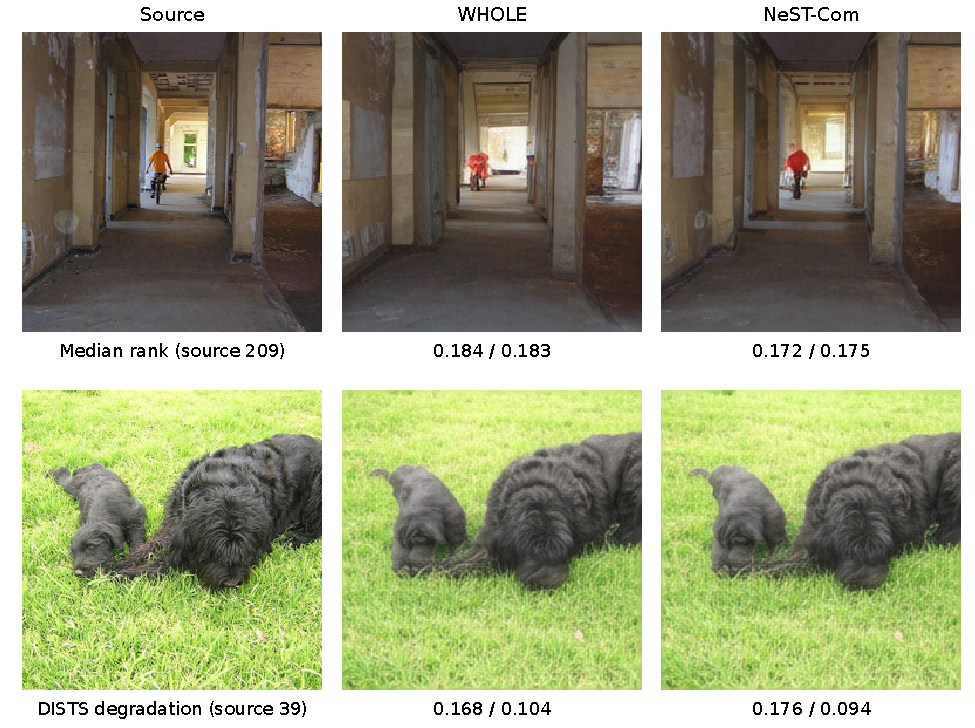
\includegraphics[width=0.80\textwidth]{figure_s1.pdf}
\caption{Uncurated reconstructions corresponding to the median (top, source~209) and minimum (bottom, source~39) source-wise DISTS gain of NeST-Com over WHOLE across the 500-image test set at $N=1024$ and 10~dB. Reported numbers denote full-image DISTS / DreamSim for the displayed realization (lower is better).}
\label{fig:s1}
\end{figure}

\end{document}
